\documentclass[margin = 10pt]{standalone}
\usepackage{xcolor}
\usepackage{tikz}
\usepackage{pgfplots}
\pgfplotsset{
compat = 1.18
}

\begin{document}
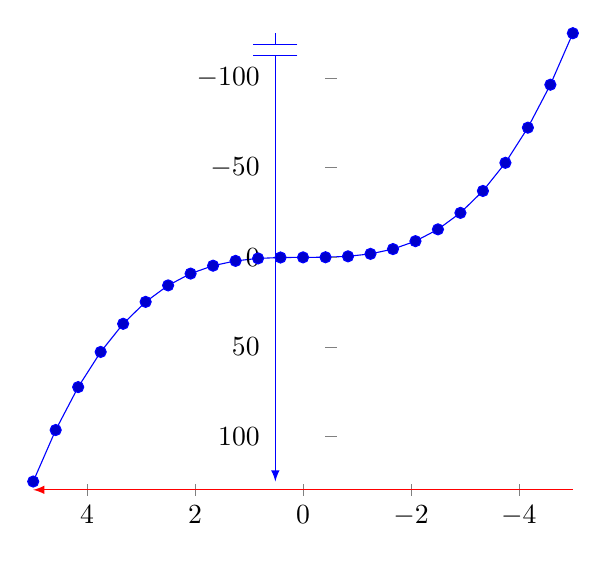
\begin{tikzpicture}[remember picture]
\begin{axis}[
    % 位置
    % box | top | middle | center | bottom | none | left | right
    axis x line = bottom,
    axis y line = middle, 
    % hide axis = true,
    axis on top,
    % 方向
    y dir = reverse,
    x dir = reverse,
    % 偏移
    axis x line shift = 3pt,
    axis y line shift = 10pt,
    % 
    % 设置轴刻度的跳跃值 crunch | parallel | none 
    % axis x discontinuity = crunch ,
    axis y discontinuity = parallel ,
    x axis line style = {-latex[],red},
    y axis line style = {-latex[],blue},
    % axis line style = {-Latex[],red},
    ]
    
    
\addplot {x^3};
\end{axis}
\end{tikzpicture}
\end{document}